%%%%%%%%%%%%%%%%%%%%%%%%%%%%%%%%%%%%%%%%%%%%%%%%%%%%%%%%%%%%%%%%%%%%%
%
% CSCI 1430 Writeup Template
%
% This is a LaTeX document. LaTeX is a markup language for producing
% documents. Your task is to fill out this
% document, then to compile this into a PDF document.
%
% TO COMPILE:
% > pdflatex thisfile.tex
%
% For references to appear correctly instead of as '??', you must run
% pdflatex twice.
%
% If you do not have LaTeX and need a LaTeX distribution:
% - Departmental machines have one installed.
% - Personal laptops (all common OS): www.latex-project.org/get/
%
% If you need help with LaTeX, please come to office hours.
% Or, there is plenty of help online:
% https://en.wikibooks.org/wiki/LaTeX
%
% Good luck!
% James and the 1430 staff
%
%%%%%%%%%%%%%%%%%%%%%%%%%%%%%%%%%%%%%%%%%%%%%%%%%%%%%%%%%%%%%%%%%%%%%
%
% How to include two graphics on the same line:
%
% \includegraphics[\width=0.49\linewidth]{yourgraphic1.png}
% \includegraphics[\width=0.49\linewidth]{yourgraphic2.png}
%
% How to include equations:
%
% \begin{equation}
% y = mx+c
% \end{equation}
%
%%%%%%%%%%%%%%%%%%%%%%%%%%%%%%%%%%%%%%%%%%%%%%%%%%%%%%%%%%%%%%%%%%%%%%%%%%%%%%%%%%%%%%%%%%%%%%%%

\documentclass[11pt]{article}

\usepackage[english]{babel}
\usepackage[utf8]{inputenc}
\usepackage[colorlinks = true,
            linkcolor = blue,
            urlcolor  = blue]{hyperref}
\usepackage[a4paper,margin=1.5in]{geometry}
\usepackage{stackengine,graphicx}
\usepackage{fancyhdr}
\setlength{\headheight}{15pt}
\usepackage{microtype}
\usepackage{times}
\usepackage{booktabs}

% python code format: https://github.com/olivierverdier/python-latex-highlighting
\usepackage{pythonhighlight}

\frenchspacing
\setlength{\parindent}{0cm} % Default is 15pt.
\setlength{\parskip}{0.3cm plus1mm minus1mm}

\pagestyle{fancy}
\fancyhf{}
\lhead{Homework Writeup}
\rhead{CSCI 1430}
\rfoot{\thepage}

\date{}

\title{\vspace{-1cm}Homework Writeup}


\begin{document}
\maketitle
\vspace{-2cm}
\thispagestyle{fancy}

\section*{Instructions}

\begin{itemize}
  \item This write-up is intended to be `light'; its function is to help us grade your work and not to be an exhaustive report.
  \item Be brief and precise.
  \item Please describe any non-standard or interesting decisions you made in writing your algorithm.
  \item Show your results and discuss any interesting findings.
  \item List any extra credit implementation and its results.
  \item Feel free to include code snippets, images, and equations. Below are useful markup templates for these.
  \item \textbf{Please make this document anonymous.}
\end{itemize}

\section*{Tasks}

\begin{itemize}
    \item \textbf{Task 1: get feature points} \\
    In get feature points, I found the gradients in x and y directions of the images through a sobel filter. Then, took the squares of the derivatives and applied a Gaussian blur. From there I used those values to calculate the cornerness score for every pixel. Then I used a threshold value of (0.1 times the maximum cornerness score value) and (half the window width) to peak local max and eliminate clusters. 
    \item \textbf{Task 2: plot feature points} \\
    For plot feature points I used plt.scatter to show where interest points are.
    \item \textbf{Task 3: get feature descriptors} \\
    For image patch, I flattened each window around the interest point to get a descriptor of dimension 256 by 1. \\
    For SIFT, I took a window around the interest point and calculated the derivatives of the window, in order to map the gradient magnitude to the feature descriptor according to its gradient orientation. After calculating each feature descriptor, I normalized the values and clamped it to less than 0.2.
    \item \textbf{Task 4: match features} \\
    I calculated the Euclidean distances between each descriptor by using numpy functions on matrices. Then sorting the distances to take the two closest points, nearest neighbor 1 (nn1) and nearest neighbor 2 (nn2). Then I used a threshold value of 0.89 to evaluate the nearest neighbor distance ratio. Values less than the threshold were valid matches. 

\end{itemize}

\section*{Result}

\begin{enumerate}
    \item First three images are of mt\_rushmore. The match features has highest accuracy: 65\%
    \item Second three images are of notre\_dame. The match features has the second highest accuracy: 65\%
    \item Last three images are of e\_gaudi. The feature matching didn't really work for this one, the accuracy was 0\%
\end{enumerate}

\begin{figure}[h]
    \centering
    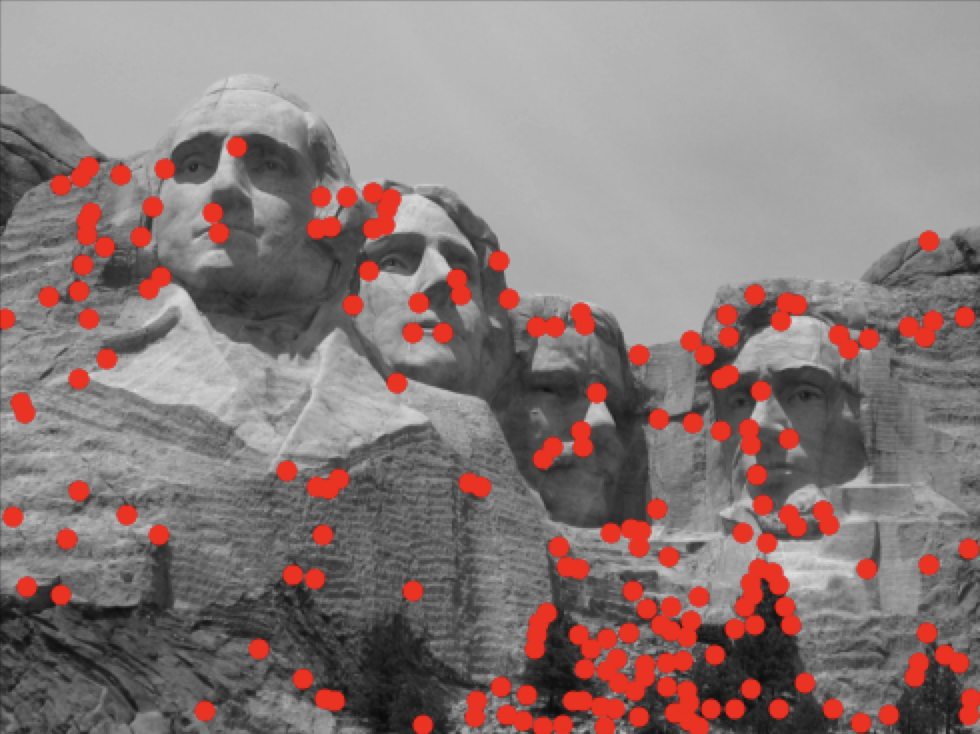
\includegraphics[width=4cm]{mt_rushmore1.png}
    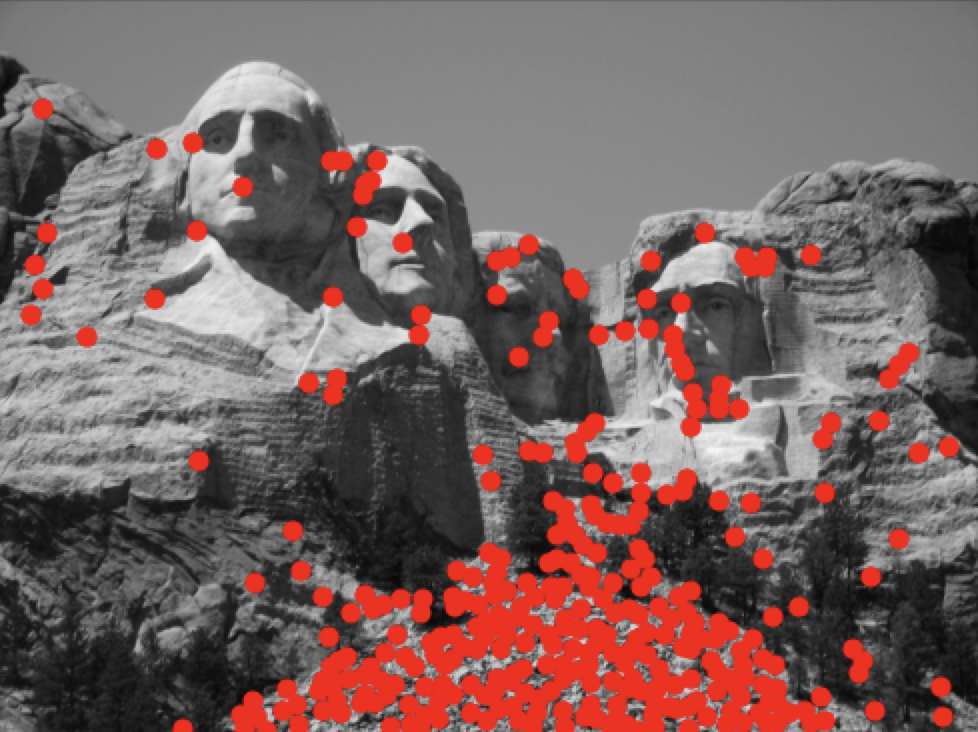
\includegraphics[width=4cm]{mt_rushmore2.png}
    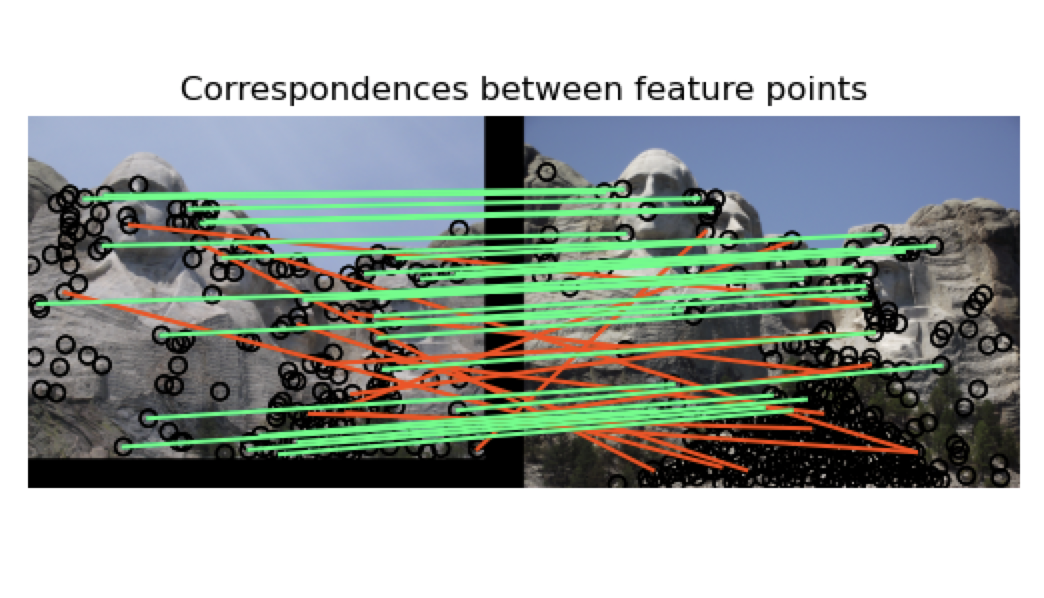
\includegraphics[width=4cm]{mt_rushmore3.png}
    \label{fig:result1}
\end{figure}

\begin{figure}[h]
    \centering
    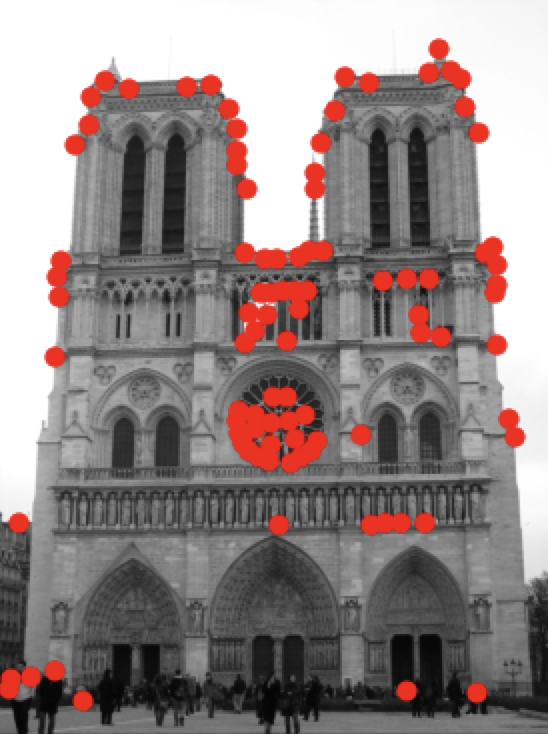
\includegraphics[width=4cm]{notre_dame1.png}
    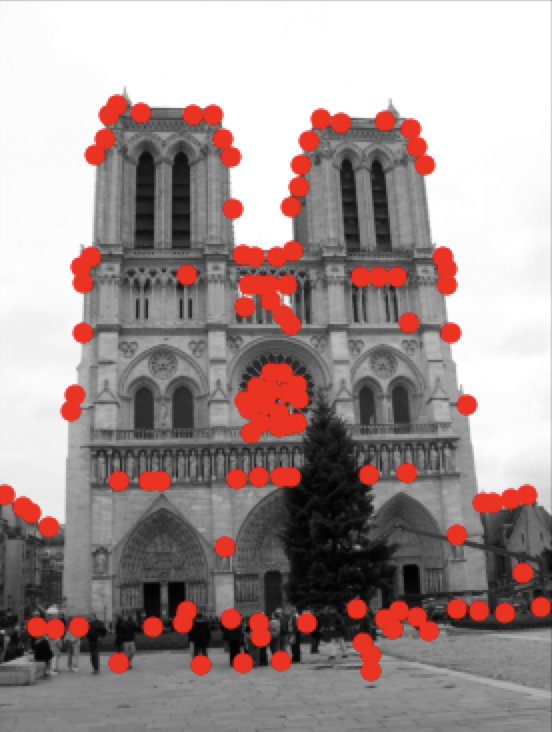
\includegraphics[width=4cm]{notre_dame2.png}
    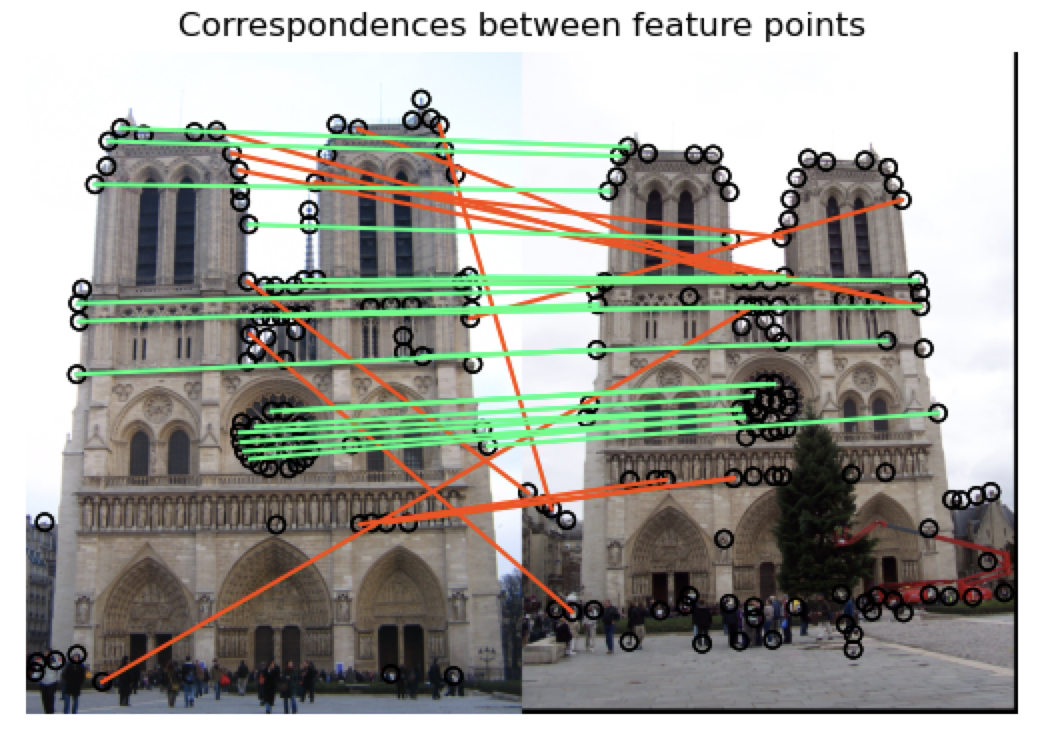
\includegraphics[width=4cm]{notre_dame3.png}
    \label{fig:result1}
\end{figure}

\begin{figure}[h]
    \centering
    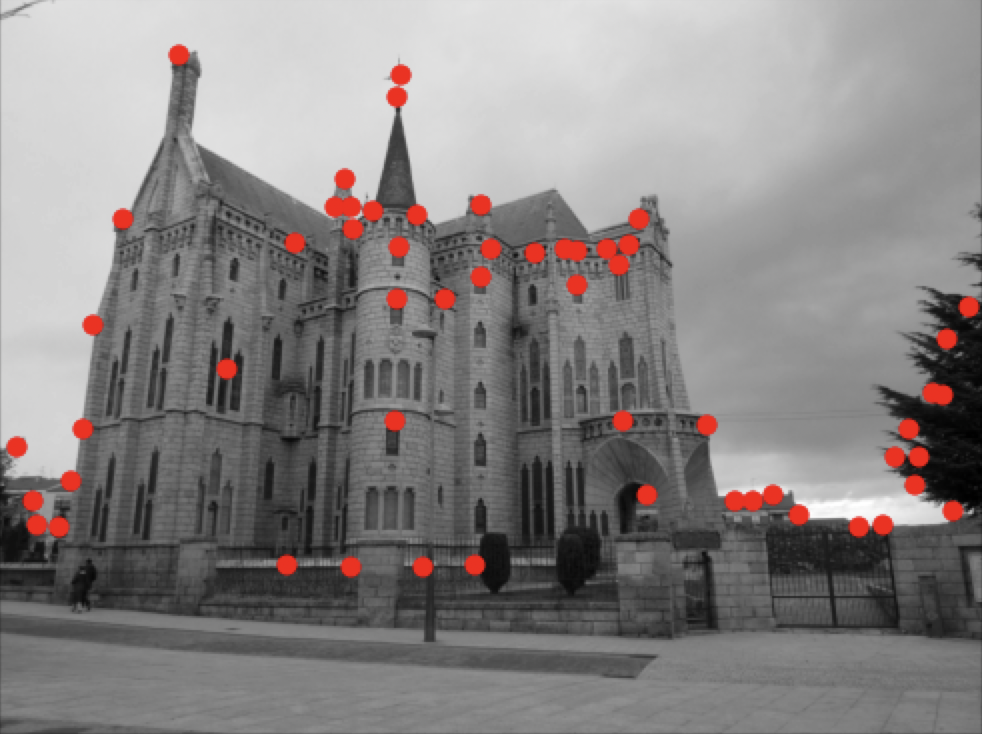
\includegraphics[width=4cm]{e_gaudi1.png}
    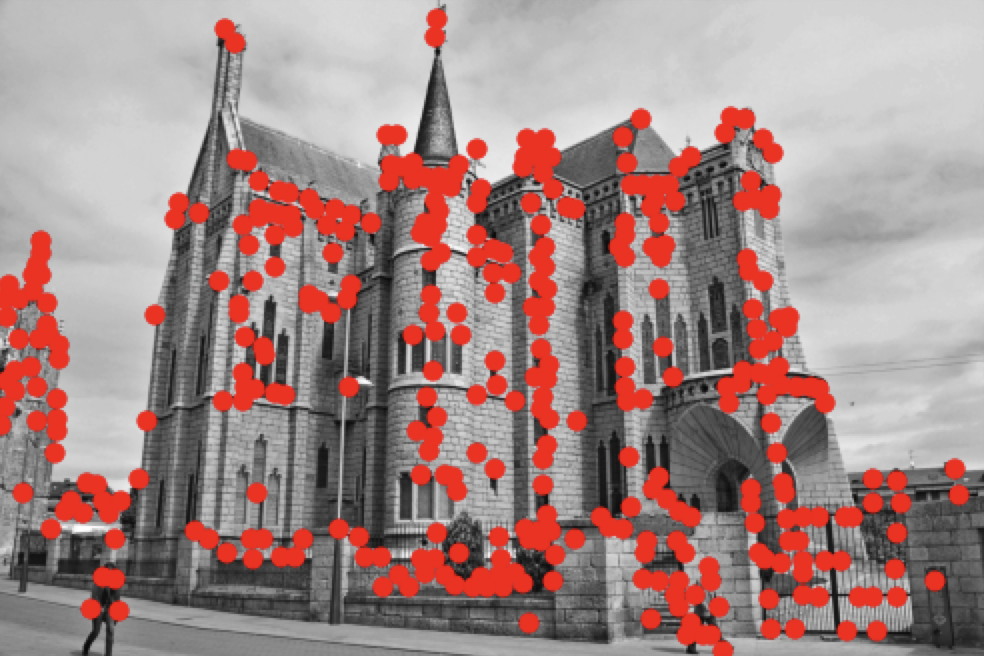
\includegraphics[width=4cm]{e_gaudi2.png}
    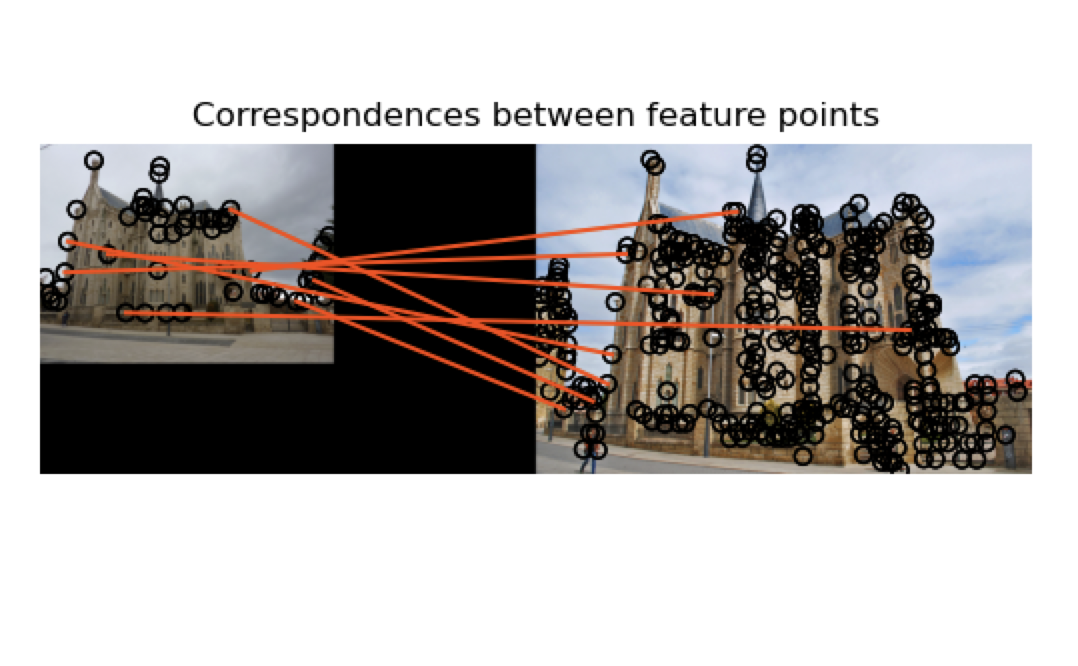
\includegraphics[width=4cm]{e_gaudi3.png}
    \label{fig:result1}
\end{figure}

\end{document}